\chapter{Demo Application}
In order to get a feeling on how to use DynamoDB we will demonstrate it by an 'real-life application' which is attached to this project. In this section a useful use-case for DynamoDB will demonstrated. Additionally it will be demonstrated that how to read and write data.

\section{Assumption}
A small company in Upper Austria is producing and selling GPS tracker for pets. These GPS tracker send a so called 'PositionReport' containing the ID of the device, a timestamp, longitude, latitude and the altitude every second. The company wants to show its users the distance covered by the pet (and therefore the tracker) on a certain range. In order to display the data we need to implement a REST service to retrieve and save data.
For the sake of convenience the REST service will be represented by a simple Java console application.

\section{Project Setup}
\subsection{Create Table in AWS}
Go to you AWS console and create a new DynamoDB table. The name of the table will be 'PositionReport'. The partition key of the table will be called 'TrackerId'. Additionally we add a sort key containing the timestamp of the report.

\begin{figure}[H]
\centering
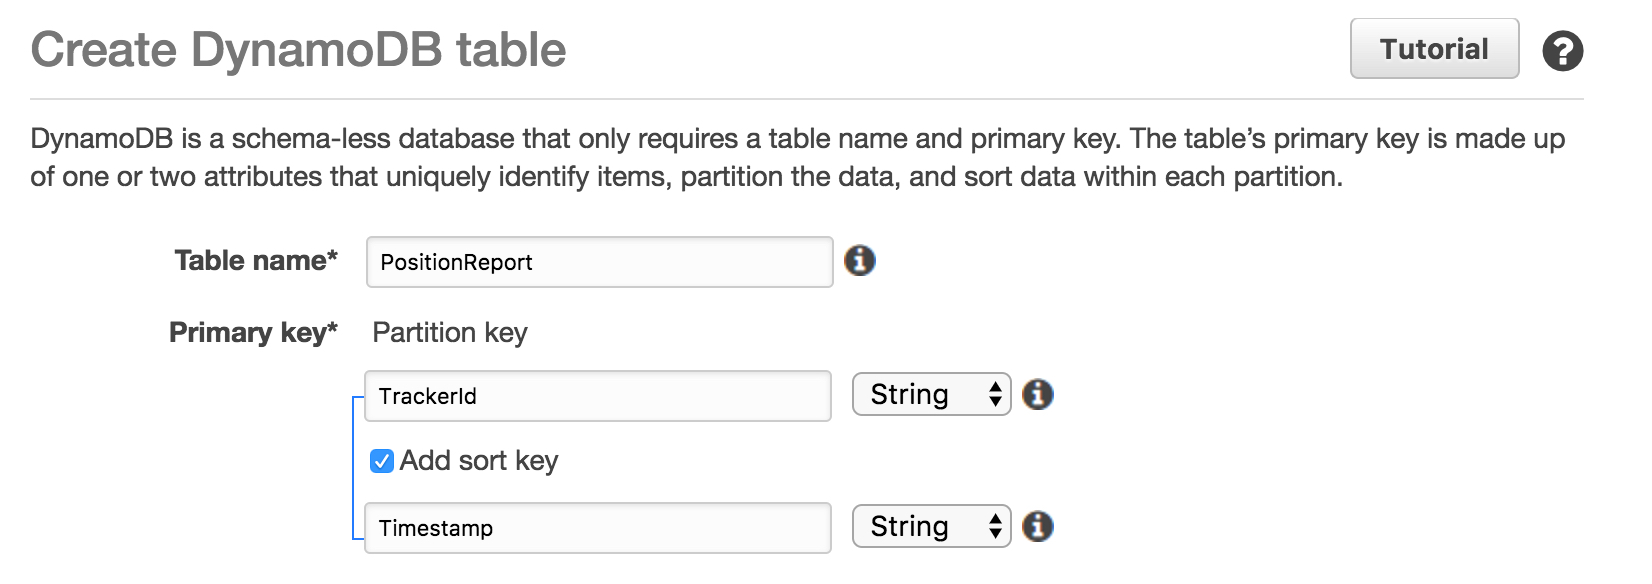
\includegraphics[width=0.9\textwidth]{images/create_table.jpg}
\caption{Creating a table in AWS.}
\end{figure}

After creating the table it takes some time until the table is ready to use.

\subsection{Adding the Credentials}
There are different ways to add the credentials for the DynamoDB. For more details on how to add the credentials go to http://docs.aws.amazon.com/sdk-for-java/v2/developer-guide/credentials.html. 

\subsection{Adding dependencies to project}
In order to use the DynamoDB API it is necessary to to install the AWS SDK and the DynamoDB SDK. These dependencies can be loaded by using a dependency manager like Apache Maven (see the following listing). 

\begin{lstlisting}
 <dependencyManagement>
        <dependencies>
            <dependency>
                <groupId>com.amazonaws</groupId>
                <artifactId>aws-java-sdk-bom</artifactId>
                <version>1.11.106</version>
                <type>pom</type>
                <scope>import</scope>
            </dependency>
        </dependencies>
    </dependencyManagement>
    <dependencies>
        <dependency>
            <groupId>com.amazonaws</groupId>
            <artifactId>aws-java-sdk-dynamodb</artifactId>
        </dependency>
        <dependency>
            <groupId>junit</groupId>
            <artifactId>junit</artifactId>
            <version>3.8.1</version>
            <scope>test</scope>
        </dependency>
    </dependencies>
\end{lstlisting}

As soon as these dependencies are loaded you're ready to start developing.

\section{Using the API}
\subsection{Connecting to AWS DynamoDB}
Before trying to connect to DynamoDB make sure that the credentials are added correctly. 

\begin{lstlisting}
DynamoDB dynamoDB = new DynamoDB(new AmazonDynamoDBClient(
	new ProfileCredentialsProvider())
);
\end{lstlisting}

\subsection{Read operation}
To be able to read a certain item you must enter the primary key. If a table also contains a sort key the sort key must also be entered. By specifying a 'projection expression' only certain attributes of a table will be selected.
\begin{lstlisting}
// select table
Table table = dynamoDB.getTable(positionReportTableName);

// read item
Item item = table.getItem(
	"TrackerId",                    // primary key name
    "ABCDEFGH",                     // primary key value
    "Timestamp",                    // sort key name
    "2017-07-14T16:34:00.638Z",     // sort key value
    "TrackerId, Altitude",     		// projection expression
    null
);

System.out.println("GetItem: printing results...");
System.out.println(item.toJSONPretty());
\end{lstlisting}

\subsection{Write operation}
The write operation is very straight forward. First of all it is necessary to select the table to write an item. Afterwards the item which should be written is created. With the method 'putItem()' the item is written to the database.
\begin{lstlisting}
// select table
Table table = dynamoDB.getTable("PositionReport");

try {
    // create item
    Item item = new Item()
        .withPrimaryKey("TrackerId", "ABCDEFGH")
        .withString("Timestamp", dateFormatter.format(new Date()))
        .withNumber("Longitude", 2)
    	.withNumber("Latitude", 500)
	    .withNumber("Altitude", 500);

	// save item
	table.putItem(item);

} catch (Exception e) {
	System.err.println("Failed to create item in " + tableName);
	System.err.println(e.getMessage());
}
\end{lstlisting}

\subsection{DynamoDB Object Mapper}
Since it is very inconvenient, error-prone and time-consuming to always create items by specifying its attribute names the DynamoDB SDK comes with an object mapper. This object mapper allows to add annotations to a POJO. In these annotations the attribute names can be specified.

\begin{lstlisting}
@DynamoDBTable(tableName="ProductCatalog")
public class PositionReport {

    @DynamoDBIndexHashKey(attributeName="Id")
    public String getTrackerId() { return trackerId; }
    public void setTrackerId(String _trackerId) { trackerId = _trackerId; }

    @DynamoDBIndexRangeKey(attributeName = "Timestamp")
    public String getTimestamp() { return timestamp; }
    public void setTimestamp(String _timestamp) { timestamp = _timestamp; }

    @DynamoDBAttribute(attributeName = "Altitude")
    public double getAltitude() { return altitude; }
    public void setAltitude(double _altitude) { altitude = _altitude; }

...
}
\end{lstlisting}
















